\section{Determine the strength of a poker hand}
\label{sec:part1}
Our first step towards developing an adaptive poker bot is to find a way to determine the strength of any given hand in any game state. In this chapter we will answer the question: 

\vspace{4mm}
\begin{statementBox2}{Problem statement 1}
How can we predict the probability of ending up with the winning hand?
\end{statementBox2}
\vspace{4mm}

Since a player do not know the outcome of the community cards during a round of poker we have to estimate odds of winning based on the possible outcomes of the community cards. It would be too time consuming to check every outcome as there are more than 250 millions different outcomes of community cards alone. Additionally, the poker rules are quite complex when it comes to determining the wining hand, therefore it is almost impossible to make a formula to calculate the exact probability. In order to find the probability without having to check the outcome of 250 million hands we need to find an estimate rather than an exact probability. 

\subsection{Design}
When trying to find an estimate we have two options.

One option is to create a simplified formula to estimate the strength of the hand. The Chen formula is an example of this. This method is straight forward but the disadvantage is that it can only be used for preflop and would limit the implementation further in the project.

Another option is to use the Monte Carlo method to simulate a lot of games and get an estimate of the probability. The Monte Carlo method is also considered to be more precise than methods similar to the it. 

For a human player the simplified formula would work best but in our case the Monte Carlo method is best suited. This is because, a computer has no problem performing calculating thousand of games, but a human would struggle to keep track of the different results from each simulation of a game. Not to mention, that a computer can calculate mathematical formulas many times faster than a human. This method also gives a trade-off between accuracy and computations which allows us to decide how accurate an estimate we need. The major poker sites also use this method to calculate the probability of ending up with the winning hand.\\

The Monte Carlo method has been implemented in as a subsystem in a playable poker game to perform the simulations and return the probability of winning given a set of hole cards. We will refer to this subsystem as the calculator. The calculator takes three arguments: the hole cards of the player, the community cards (optional) and the number of opponents. The calculator then performs the simulations and returns an object containing the distribution of outcomes.
Caniwin~\cite{caniwin} is a website that has calculated the probability of winning with each of the 169 different hole cards combination. We consider caniwins results to be the actual probability of winning with a given combination of hole cards. This sites results is limted to the preflop game state, but is still a good indicator to prove that the Monte Carlo method has been implemented correctly.

Requirements for the calculator:
\begin{itemize}
\item It shall be able to return the probability of winning for any poker game state with up to ten players.
\item It must have a maximum error percentage of one percent. (deviation from caniwin)
\item It shall calculate the probability in less than five seconds.
\end{itemize}


\subsubsection{Monte Carlo method}
The Monte Carlo method can be used to calculate a distribution of results for any given set of hole cards. The system developed were given a specific combination of hole cards to calculate an estimate, on what the probability of winning with that hand was. The Monte Carlo simulation then ran x number of games with the same hand, each time giving the opponents a random set of hole cards. The distribution of results we get can be used to find the likelihood of possible outcomes by looking at how many wins and loses compared to the number of games. The more simulations that are performed the more accurate the probabilities will get when comparing to caniwins results.

\subsection{Test}
To test if the calculator can calculates the correct probabilities we find the probability of a number of different pre-flop scenarios and compare the result with the results of caniwin. Every test have been preformed with 50.000 simulations against one opponent. The result can be seen in table \ref{tab:pre-flop-test}. From the results we can see that for all hole cards the error percentage is less than one.

To test the accuracy of the calculator we try to find a number of simulations that fulfil the requirements. This is done by comparing the error percentage we get with a different number of simulations. Each test is performed with a pair of jacks in pre-flop with one opponent. Caniwin found the probability to be 77,1 \%. Figure~\ref{fig:mc1}, \ref{fig:mc10} and \ref{fig:mc50} shows the distribution of results from 50 tests. Each test result is indicated with a red dot. In figure~\ref{fig:mc1} we can see the results ranges from 74,4 \% to 79,6 \% (5,2 \%). In figure~\ref{fig:mc10} the range is only 75,7 \% to 77,9 \% (2,2 \%) and finally in figure~\ref{fig:mc50} the range is down to 76,4 \% to 77,3 \% (0,9 \%).

In table \ref{tab:mc-total} you can see the combined result. The range is the difference between the lowest and highest result and the max error is the maximum deviation from caniwin.



\begin{figure}[H]
  \center
    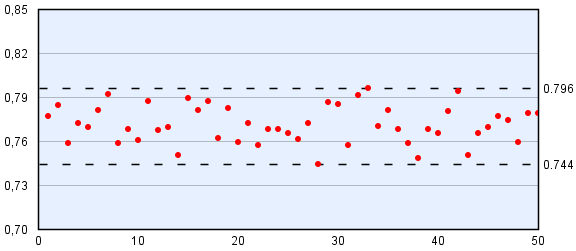
\includegraphics[scale=0.775]{images/MonteCarlo/1k.png}
  \caption{Result of the calculator with 1000 simulations \label{fig:mc1}}
\end{figure}

\begin{figure}[H]
  \center
    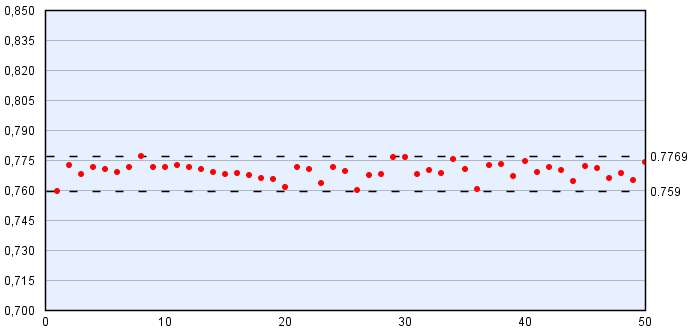
\includegraphics[scale=0.775]{images/MonteCarlo/10k.png}
  \caption{Result of the calculator with 10.000 simulations \label{fig:mc10}}
\end{figure}

\begin{figure}[H]
  \center
    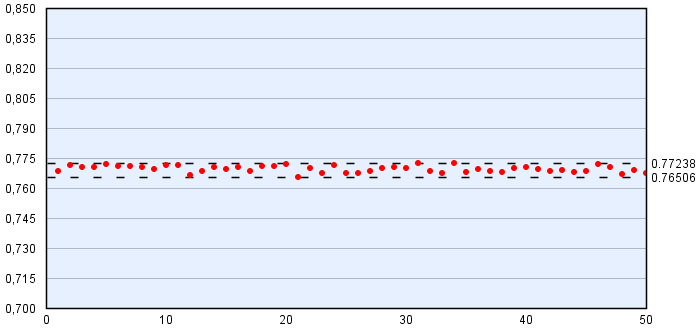
\includegraphics[scale=0.775]{images/MonteCarlo/50k.png}
  \caption{Result of the calculator with 50.000 simulations \label{fig:mc50}}
\end{figure}

The three graphs clearly states that when using a higher amount of simulations, the more accurate the probability will become.
The error percentage in table 2 have been calculate by comparing the calculators results to caniwin: \[Our result - caniwin\]
We settled for 50.000 as the number of simulations for our calculator. This satisfies our requirements..

\vspace{4mm}
\def\arraystretch{1.5}
\begin{table}[H]
  \center
  \begin{tabular}{ | l | l | l | l | }
  	\hline
  	hole cards & our result (\%) & caniwin (\%) & error (\%) \\
  	\hline                       
    A\clubsuit ~ A\diamondsuit & 85,2 & 84,9 & 0,3 \\
    8\clubsuit ~ 8\diamondsuit & 67,9 & 68,7 & 0,8 \\
    Q\clubsuit ~ k\clubsuit & 62,8 & 62,4 & 0,4 \\
    A\heartsuit ~ 8\spadesuit & 58,8 & 60,5 & 0,7 \\
    J\spadesuit ~ Q\diamondsuit & 57,2 & 56,9 & 0,3 \\
    10\heartsuit ~ J\heartsuit & 56,7 & 56,2 & 0,5 \\
    3\diamondsuit ~ 3\spadesuit & 53,0 & 52,8 & 0,2 \\
    2\diamondsuit ~ 2\heartsuit & 49,5 & 49,4 & 0,1 \\
    9\diamondsuit ~ 3\spadesuit & 37,8 & 37,4 & 0,4 \\
    2\diamondsuit ~ 7\diamondsuit & 35,5 & 35,4 & 0,1 \\
    2\diamondsuit ~ 7\heartsuit & 31,9 & 31,7 & 0,2 \\
  	\hline   	
  \end{tabular}
  \caption{Test results for different hole cards in pre-flop with one opponent \label{tab:pre-flop-test}}
\end{table}
\vspace{4mm} 

\vspace{4mm}
\begin{table}[H]
  \center
  \begin{tabular}{ | l | l | l | l | }
    \hline
    simulations & range (\%) & max error (\%) & time (seconds) \\
    \hline                       
    1000 & 5,2 & 2,7 & 0,03 \\
    10.000 & 2,2 & 1,5 & 0,22\\
    50.000 & 0,9 & 0,7 & 0,82\\
  \hline  
  \end{tabular}
  \caption{Combined test results from running the calculator with different numbers of simulations. \label{tab:mc-total}}
\end{table}
\vspace{4mm}

\subsection{Discussion}
For the implementation of the calculator the Monte Carlo method was. This method works well for the needs. The calculator can calculate the probability with an error percentage of less than one percent when using 50.000 simulations. This solution can be used for any poker state with up to ten players. At first it did not seem necessary to optimise the calculator any further, as the running time is acceptable. But in regards to later use or if were to scale the project, we decided to make an obvious optimisation by making it multi-threaded which speeded up the calculations by..................

Alternatively we could have created our own formula to calculate a rank, or used an existing one, for instance the Chen formula. By using this method we will get a less accurate result but it will be easier to calculate. We would also have to create a formula for each game state which would cause even more work. Since performance is not a problem for our calculator we chose to use the Monte Carlo method.

\subsection{Conclusion}
In this section we have answered the question:
\vspace{4mm}
\begin{statementBox2}{Problem statement 1}
How can we predict the probability of ending up with the winning hand?
\end{statementBox2}
\vspace{4mm}

We have implemented a subsystem called the calculator that can estimate the probability of winning with a set of hole cards. The calculator uses the Monte Carlo method and it works for every poker state with up to ten players. We have found that 50.000 simulations is a good number of simulations for our calculator. 

We compare our results to caniwin, which is a website that calculates the actual probabilities of all the 169 combinations of hole cards. The calculator has a maximal error percentage of one percent and performs the simulation in less than a second.